\section{Implementation}\label{sec:implementation}

The original MINAS algorithm has a companion implementation (\refminas)
written in Java using MOA library base algorithms such as K-means and CluStream.
% \refminas employs Java's double, a $64 bits$ number whose precision is not
% absolutely necessary and, as it is often necessary to shuffle between nodes via
% network and a small economy could be made with only a float number with $32 bits$.
Another difference between \refminas and \mfog is cluster radius calculation
from the distances of elements forming the cluster and the cluster's center,
where the former uses the maximum distance, the latter uses the standard deviation
of all distances as described in \cite{Faria2016minas}.

\begin{figure}[htb]
\centerline{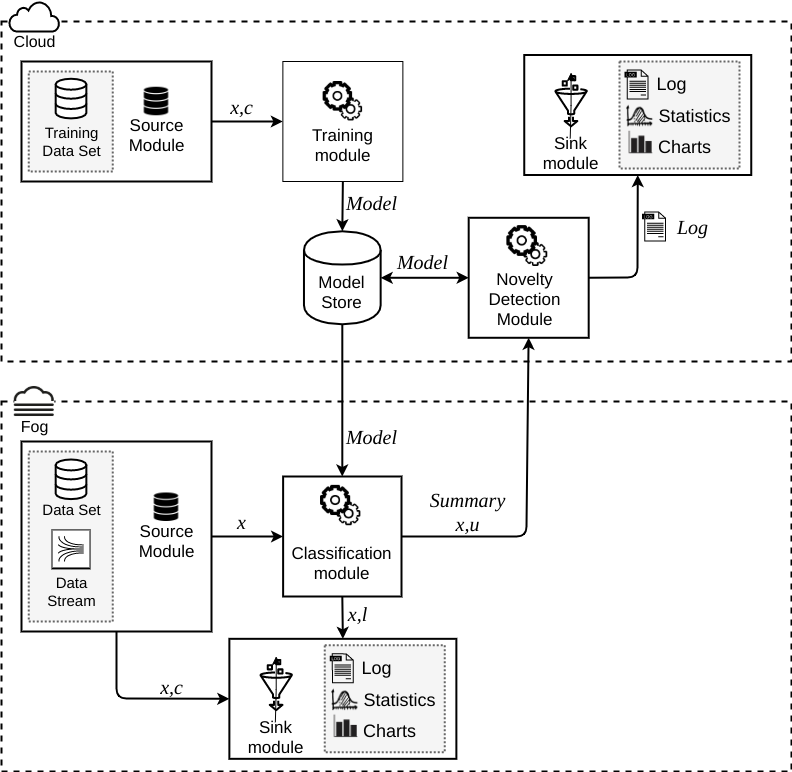
\includegraphics[width=0.5\textwidth]{figures/mfog-arch-v2_en.png}}
\caption{\mfog architecture overview.}
\label{fig:mfog-architecture}
\end{figure}

% Desafios de implementação:
% <!--
% - Definição de raio: desvio padrão das distâncias versus distancia máxima;
% - Atualização do micro-cluster limita-se à atualização do atributo \texttt{T};
% - Remoção de exemplos na implementação de referência é feita somente para o algoritmo \textit{CluStream};
% - Inclusão de borda: algoritmo inclui ($<=$), referência não inclui ($<$);
% - Seguiu-se as mesmas divergências anteriores para comparação dos resultados com a implementação referência;
% - Inclusão da borda;
% - Comportamento do mecânismo de \textit{sleep-model} não está definido, portanto não está ativo;
% - Processo de clusterização é limitado ao algoritmo \textit{K-Means}. Algoritmo \textit{CluStream} não está implementado;
% - -->
% - `Double vs Float`:
%   - Na implementação de referência, java double é utilizado;
%   - Na nova implementação duas versões foram testadas e a diferença de precisão entre as duas é de `5 E-8`;
%   - **Solução:** Use `float32` e economize os bits já que haverá comunicação entre nós e módulos;
% - Formato do fluxo de saída:
%   - Implementação de referência utiliza a tripla `(id, classe, etiqueta)`;
%   - Primeira implementação em C utiliza `(id, clusterLabel, clusterId, clusterRadius, label, distance, secondDistance)`;
%   - Segunda implementação utiliza dupla `(id, label)`;
%   - Na etapa de avaliação, independente de versão, o fluxo original é lido;
%   - **Solução:** O formato mínimo é `(id, label)`;

The stream format for input and output also of note.
Input information needed is the value of the item, this value is a number
sequence of length $d$ (referenced as dimension).
In addition to the value for evaluation and training purposes the class
identifier as single character, optimality an unique item identifier
(\textit{uid}) can be provided.
For output information and format the decision isn't so clear as we can't
predict future system integrations needs like only novelty alarms or every
item's original value with assigned label so, we have a compromise and put only
enough information for the Evaluation Module (where the full information
from the testing file or stream can de accessed) meaning the format can be
defined as a tuple containing \textit{uid} and assigned label.

% - Reprocessamento dos exemplos utilizados para atualização do modelo:
%   - Muda o comportamento do operador de fluxo de `Map` para `Flatmap`, ou seja,
%     requer outro fluxo de saída para a transmissão de padrões novidade (alarmes);
%   - Para reclassificação a definição de raio é modificada de `r = f * σ` (fator
%     multiplicando desvio padrão) para `r = max(distance)` (distância máxima);
%   - Passível da crítica de *overfitting*. Isto é, este processo pode
%     inflar a métrica de precisão;
%   - **Solução:** *em aberto*;

Another implementation decision related to the output stream is whether or not
to reprocess, and add to the output stream, examples in the unknown buffer after
the novelty detection procedure, meaning one item can be classified once as
unknown and again with a label.
Our tests using this technique had increased true positives when compared to
not using it.
However this changes the stream operator behavior from a \textit{Map} to a
\textit{FlatMap} having duplicate entries on the output stream as previously
mentioned.
Regardless of choice the classification of the unknown buffer after a model
update, using the full model or just the added set of clusters, is done to
remove the examples ``consumed'' in the creation of a new cluster in the internals
of the clustering algorithm.
% This removal can be made less complex if using only new clusters 

% Próximos desafios:
% - Distribuição e paralelização para minimização de latência entre novo item no fluxo e sua classificação:
%   - Tempo de passagem da instância pelo classificador;
%   - Volume máximo do sistema;
%   - Diferenças de precisão de acordo com a carga;

For \mfog the Message Passing Interface (MPI) library was used.
In MPI programming, multiple processes of the same program are created by the
runtime and each process instance receives a rank parameter, for \mfog this
parameters indicate if the process is root, rank $0$, or leaf otherwise.
Beyond this division, each process also operates two threads, for the root
there is a sampler and detector threads, for the leafs each has a model receiver
thread and multiple classifier threads.
The overall sequence of creation is shown in \reffig{mfog-mpi-life}.

\begin{figure}[htb]
  \centerline{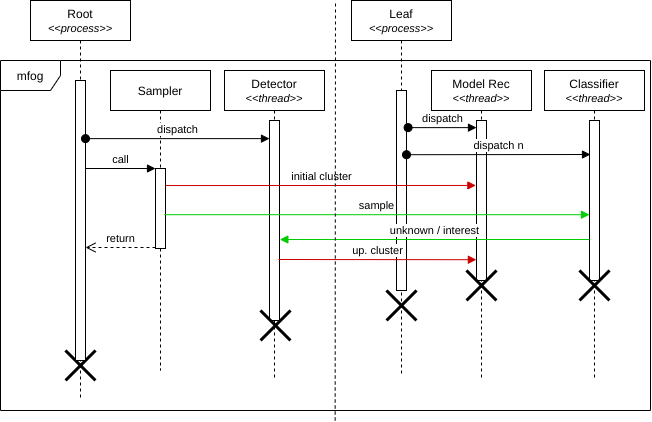
\includegraphics[width=0.5\textwidth]{figures/mfog-arch-mpi.png}}
  \caption{\mfog life line overview.}
  \label{fig:mfog-mpi-life}
\end{figure}

\begin{highlight}
Polices

- Detecção de novidades e manutenção de modelo em ambiente distribuído:

  - Mecanismo de ND local (síncrono) vs nuvem quanto à atraso de definição de modelo
    (nesse ponto é onde a hipótese prevê maior diferença, grande ponto de interesse);

  - Mecanismo de esquecimento local vs global (modelo único ou por nó);

  - Atraso na reclassificação dos desconhecidos;
\end{highlight}

The Evaluation Module was also build following reference techniques like
multi-class confusion matrix with label-class association
\cite{Faria2016minas}
to extract classification quality metrics.